\documentclass[letterpaper]{article}
\usepackage[margin=1in]{geometry}
\usepackage[utf8]{inputenc}
\usepackage{textcomp}
\usepackage{amssymb}
\usepackage{natbib}
\usepackage{graphicx}
\usepackage{gensymb}
\usepackage{amsthm, amsmath, mathtools}
\usepackage[dvipsnames]{xcolor}
\usepackage{enumerate}
\usepackage{mdframed}
\usepackage[most]{tcolorbox}
\usepackage{csquotes}
% https://tex.stackexchange.com/questions/13506/how-to-continue-the-framed-text-box-on-multiple-pages

\tcbuselibrary{theorems}

\newcommand{\R}{\mathbb{R}}
\newcommand{\Z}{\mathbb{Z}}
\newcommand{\N}{\mathbb{N}}
\newcommand{\Q}{\mathbb{Q}}
\newcommand{\C}{\mathbb{C}}
\newcommand{\code}[1]{\texttt{#1}}
\newcommand{\mdiamond}{$\diamondsuit$}
\newcommand{\PowerSet}{\mathcal{P}}
\newcommand{\Mod}[1]{\ (\mathrm{mod}\ #1)}
\DeclareMathOperator{\lcm}{lcm}

%\newtheorem*{theorem}{Theorem}
%\newtheorem*{definition}{Definition}
%\newtheorem*{corollary}{Corollary}
%\newtheorem*{lemma}{Lemma}
\newtheorem*{proposition}{Proposition}


\newtcbtheorem[number within=section]{theorem}{Theorem}
{colback=green!5,colframe=green!35!black,fonttitle=\bfseries}{th}

\newtcbtheorem[number within=section]{definition}{Definition}
{colback=blue!5,colframe=blue!35!black,fonttitle=\bfseries}{def}

\newtcbtheorem[number within=section]{corollary}{Corollary}
{colback=yellow!5,colframe=yellow!35!black,fonttitle=\bfseries}{cor}

\newtcbtheorem[number within=section]{lemma}{Lemma}
{colback=red!5,colframe=red!35!black,fonttitle=\bfseries}{lem}

\newtcbtheorem[number within=section]{example}{Example}
{colback=white!5,colframe=white!35!black,fonttitle=\bfseries}{def}

\newtcbtheorem[number within=section]{note}{Important Note}{
        enhanced,
        sharp corners,
        attach boxed title to top left={
            xshift=-1mm,
            yshift=-5mm,
            yshifttext=-1mm
        },
        top=1.5em,
        colback=white,
        colframe=black,
        fonttitle=\bfseries,
        boxed title style={
            sharp corners,
            size=small,
            colback=red!75!black,
            colframe=red!75!black,
        } 
    }{impnote}
\usepackage[utf8]{inputenc}
\usepackage[english]{babel}
\usepackage{fancyhdr}
\usepackage[hidelinks]{hyperref}

\pagestyle{fancy}
\fancyhf{}
\rhead{Math 170B}
\chead{Wednesday, May 31, 2023 \& Friday, June 02, 2023}
\lhead{Lecture 26}
\rfoot{\thepage}

\setlength{\parindent}{0pt}

\begin{document}

\section{Simulated Annealing (Section 11.6)}
This is typically an algorithm for a discrete search. This particular algoritihm does not use derivatives, either. 

\begin{mdframed}
    (Example: Traveling Salesperson.) The problem statement is as follows: Suppose we have a network of different cities. Our goal is to find the minimum cost to visit each city once (and only once).

    \begin{center}
        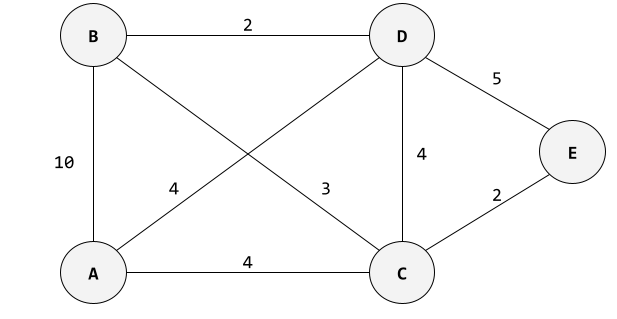
\includegraphics[scale=0.5]{../assets/traveling_salesperson.png}
    \end{center}

    For large networks, multiple local minima may exists.
\end{mdframed}

\subsection{A Brute Force Approach}
Suppose $F(x): \R^n \to \R$ represents the cost of traveling a particular route. The simulated annealing also uses random components. At iteration $k$, given $F(x^{(k)})$ and $m$, we want to generate candidates $u_1, u_2, u_3, \hdots, u_m \in \R^n$. This is typically done by random process: in the traveling salesperson problem, we consider the different edges we could take. By evaluating the function at each candidate point, we can find \emph{one} of them that has the least cost; that is, 
\[u_j = \min_{1 \leq i \leq m} F(u_i).\]
If $F(u_j) \leq F(x^{(k)})$, then we can update the iterate, \[x^{(k + 1)} = u_j.\]
Otherwise, we can do the following: 
\begin{itemize}
    \item Compute the probability for each $u_i$,
    \[\tilde{p}_i = e^{\alpha (F(x^{(k)}) - F(u_i))} \qquad q \leq i \leq m, \quad \alpha > 0, \quad \tilde{p}_i \in \R.\]

    \item Rescale (normalize) the probability,
    \[\tilde{p}_i = \frac{\tilde{p}_i}{\sum_{k = 1}^{m} \tilde{p}_k}.\]

    \item For a random uniformly distributed variable $\rho \in [0, 1]$, we want to find the index $\ell$ such that 
    \[\tilde{p}_1 + \tilde{p}_2 + \hdots + \tilde{p}_{\ell - 1} \leq \rho \leq \tilde{p}_1 + \tilde{p}_2 + \hdots + \tilde{p}_{\ell - 1} + \tilde{p}_{\ell}.\]
    Based on the index, we have 
    \[x^{(k + 1)} = u_{\ell}.\]
\end{itemize}


\subsection{Coordinate Descent \& Pattern Search}
This method is somewhat similar to the Nelder-Mead method. It also does not use derivatives. Coordinate descent aims to minimize one variable at a time, when $F: \R^n \to \R$. The idea is to cycle through the $m$ coordinate directions, corresponding to $e_1, e_2, \hdots, e_n$. Recall that $e_i = \begin{bmatrix}
    0 \\ \vdots \\ 0 \\ 1 \\ 0 \\ \vdots \\ 0
\end{bmatrix}$, with the 1 being in the $i$th position. We want to line-search along each coordinate direction. The iteration relies on the finding of $\alpha_k$, 
\[\alpha_k = \min_{\alpha} F(x^{(k)} + \alpha e_k).\]
From there, \[x^{(k + 1)} = x^{(k)} + \alpha_k e_k \qquad k = 1, 2, \hdots.\]
When $k = 1$, we count forward. When $k = m$, we count backwards. So, we would do something like 
\[e_1, e_2, \hdots, e_{n - 1}, e_n, e_{n - 1}, e_{n - 2}, \hdots, e_2, e_1, e_2, \hdots\]
One modification we can do to this process is to search along a line after a few iterations of the method. However, this modification converges pretty slowly. 

\subsection{Pattern Search}
We can incorporate pattern-search methods to generalize coordinate descent. Suppose there is a set of directions, $p_k \in D_k$. Here, $D_k$ is called the \emph{direction set}, and $p_k$ is an $n \times 1$ vector representing a direction. The pattern-search methods are not only dependent on the direction vector, but also a fixed step size $\alpha_k$. 

\bigskip 

To update $\alpha_k$, we'll consider a \emph{frame} of all directions. We'll update the current value by considering every direction. The frame is defined by 
\[x^{(k)} + \alpha_k p_k, \qquad p_k \in D_k.\]

\begin{mdframed}
    (Example.) Suppose our direction set is defined by 
    \[D_{k} = \left\{p_i : 1 \leq i \leq n\right\} \cup \{p_{n + 1}\},\]
    with $p_i = \frac{1}{2m}e - e_i$; and, $p_{n + 1} = \frac{1}{2m} e$. This is known as the simplex direction set, and its frame looks like 
    \begin{center}
        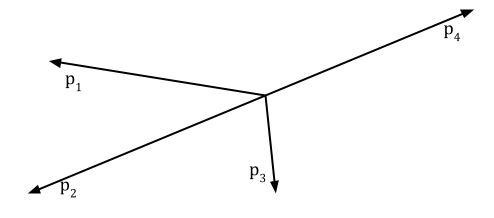
\includegraphics[scale=0.5]{../assets/simplex_directions.png}
    \end{center}
\end{mdframed}

\begin{mdframed}
    (Example.) In $\R^3$, suppose our direction set is \[D_{k} = \{e_1, e_2, e_3, -e_1, -e_2, -e_3\}.\] Then, our frame is defined by 
    \begin{center}
        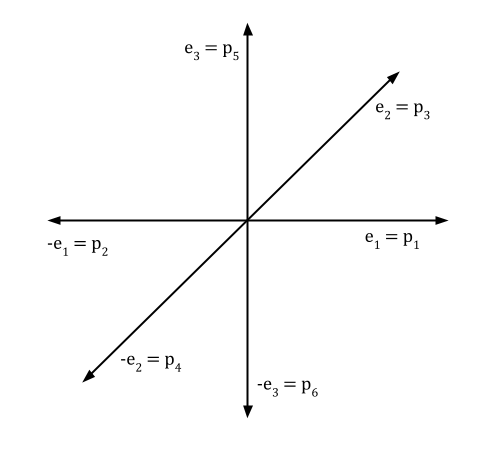
\includegraphics[scale=0.5]{../assets/coordinate_descent.png}
    \end{center}
\end{mdframed}
The corresponding algorithm takes the following arguments
\begin{itemize}
    \item $\epsilon > 0$, the tolerance,
    \item $1 > \beta > 0$, the contraction, 
    \item $\alpha > \epsilon$, 
    \item $\gamma \geq 1$, the expansion 
    \item $D_0$, the initial direction set,
    \item $M \geq 0$, the reduction measure.  
\end{itemize}

\begin{algorithm}[H]
    \caption{Pattern Search Method}
    \begin{algorithmic}[1]
        \Function{PatternSearch}{$\epsilon, \beta, \alpha, \gamma, D_0, M$}
            \For{$k \gets 1$ to $\infty$}
                \If{$\alpha \leq \epsilon$}
                    \State break 
                \EndIf 

                \If{$F(x^{(k)} + \alpha) < F(x^{(k)}) - M\alpha^3$}
                    \State $p_k \in D_k$ 
                    \State $x^{({k + 1})} \gets x^{(k)} + \alpha p_{k}$ \Comment{For some such $p_k$}
                    \State $\alpha \gets \gamma \alpha$
                \Else 
                    \State $x^{(k + 1)} \gets x^{(k)}$
                    \State $\alpha \gets \beta \alpha$
                \EndIf 
            \EndFor 
        \EndFunction 
    \end{algorithmic}
\end{algorithm}


\subsection{Line Search}
Recall that the line search was used for selecting the step length. In this context, we'll say that the updates of solution estimates are of the form 
\[x^{(k + 1)} = x^{(k)} + \alpha_{k} p_{k},\]
where $\alpha_{k}$ is a scalar representing the step length and $p_{k}$ is a vector representing the direction. To determine a step length, typically a 1D search is done. Given a direction $p_k$ and $F(x): \R^n \to \R$, $\phi: \R \to \R$, we have 
\[\phi(\alpha) = F(x^{(k)} + \alpha p_k)\]
\[\phi'(\alpha) = p_{k}^T \nabla F(x^{(k)} + \alpha p_k).\]
Note that $p_k$ should be a descent direction; that is, $p_k^T \nabla F(x_k) \leq 0$. Now, to minimize $\phi$ (i.e., to approximate $\min_{\alpha > 0} \phi(\alpha)$), a set of conditions are used: 
\begin{itemize}
    \item \textbf{Condition 1:} ``Sufficient'' decrease. 
    
    \begin{mdframed}
        (Example.) Note that $F(x^{(k + 1)}) < F(x^{(k)})$ alone isn't enough for this condition. To see why, consider $F(x) = x^2 - 1$. Suppose we have a sequence $\{x_k\}$ so that $F(x_{k}) = 4/k$. 
        \begin{center}
            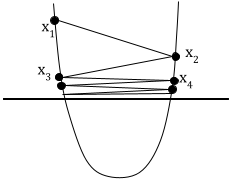
\includegraphics[scale=0.7]{../assets/cond_dec.png}
        \end{center}
        Notice that $F(x_{k + 1}) < F(x_{k})$, but the result does not converge to the minimum.
    \end{mdframed}
    With this example in mind, a sufficient decrease is one that satisfies 
    \[\phi(\alpha_k) \leq \phi(0) + \alpha_k c_1 \phi'(0)\]
    \[F(x^{(k)} + \alpha_k p_k) \leq F(x^{(k)}) + \alpha_k c_1 \nabla F^{T}(x^{(k)}) p_k.\]
    Here, $c_1 \in (0, 1)$ is some parameter, with the most common value being $c_1 = 10^{-4}$; this means that the line often looks flat. Visually, this looks like 
    \begin{center}
        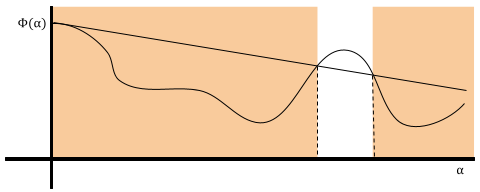
\includegraphics[scale=0.7]{../assets/line_search_dec.png}
    \end{center} 
    The orange region denotes a sufficient decrease (where $\phi$ is less than or equal to the value of the line). The line can be defined by $\ell(\alpha) = \phi(0) + \alpha c_1 \phi'(0)$. Note that the step $\alpha$ may be very small.
    
    \item \textbf{Condition 2:} Curvature condition. In particular, we have 
    \[|\phi'(\alpha_k) \leq c_2 |\phi'(0)|, \qquad c_2 \in (c_1, 1).\]
\end{itemize}
With this in mind, we'll introduce the \textbf{Wolfe-Conditions}, which is essentially a combination of the above two conditions. For step lengths, we have \[F(x^{(k)} + \alpha p_k) \leq F(x^{(k)}) + c_1 \alpha \nabla F(x^{(k)})^T p_k,\]
\[|\nabla F(x^{(k)} + \alpha p_k)^T p_k| \leq c_2 |\nabla F(x^{(k)})^T p_k|.\]
Visually, we want to add tangent lines to the points corresponding to $c_2 |\phi'(0)| \geq |\phi'(\alpha)|$.
\begin{center}
    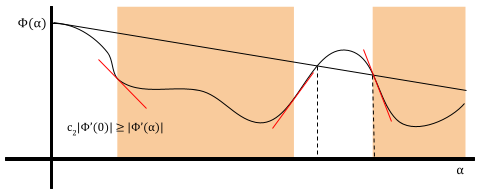
\includegraphics[scale=0.7]{../assets/line_search_dec2.png}
\end{center}
Here, the orange region denotes the region satisfied by the Wolfe-Condition. Wolfe line search is effective in practice, but generally difficult to implement. 

\subsubsection{Armijo Line Search}
A generally effective simple line search method is the Armijo Search, also known as a backtracking line search. This is for a sufficient decrease, where the step size is not too small. In particular, for $\alpha = 1 > 0$, $c_1 = 10^{-4}$, and $\rho = \frac{1}{2}$, we have 
\begin{algorithm}[H]
    \caption{Armijo Line Search}
    \begin{algorithmic}[1]
        \While{$F(x^{(k)} + \alpha p_k) > F(x^{(k)}) + c_1 \alpha \nabla F(x^{(k)})^T p_k$}
            \State $\alpha \gets \rho \alpha$
        \EndWhile 
    \end{algorithmic}
\end{algorithm}

\subsubsection{Wolfe Line Search}
The Wolfe Line Search algorithm has the following arguments: 
\begin{itemize}
    \item $\alpha_0 = 0$
    \item $\alpha_{\max} > 0$ (e.g., 100)
    \item $\alpha_1 \in (0, \alpha_{\max})$ (e.g., 1)
    \item $c_1 = 0.9$
    \item $c_2 = 10^{-4}$
\end{itemize}
\begin{algorithm}[H]
    \caption{Wolfe Line Search}
    \begin{algorithmic}[1]
        \Function{Wolfe}{$\alpha_i, \alpha_{\max}, c_1, c_2$}
            \State $i \gets 0$
            \While{true} 
                \If{$\phi(\alpha_i) > \phi(0) + c_1 \alpha_i \phi'(0)$ or $\phi(\alpha_i) \geq \phi(\alpha_{i - 1})$ and $i > 1$}
                    \State $\alpha^* \gets \text{zoom}(\alpha_{i - 1}, \alpha_{i})$
                    \State break 
                \EndIf 

                \If{$\phi'(\alpha_i) \geq 0$}
                    \State $\alpha^* = \text{zoom}(\alpha_i, \alpha_{i - 1})$
                    \State break 
                \EndIf 

                \State $\alpha_{i + 1} \gets 2 \alpha_i$
                \State $i \gets i + 1$
            \EndWhile 

            \State $\text{zoom}(\alpha_{\text{low}}, \alpha_{\text{high}})$
            \While{true} 
                \State $\alpha_j = \frac{1}{2}(\alpha_{\text{low}} + \alpha_{\text{high}})$
                \If{$\phi(\alpha_j) > \phi(0) + c_1 \alpha_j \phi'(0)$ or $\phi(\alpha_j) \geq \phi(\alpha_{\text{low}})$}
                    \State $\alpha_{\text{high}} \gets \alpha_j$
                \Else 
                    \If{$\phi'(\alpha_j)| \leq -c_2 \phi'(0)$}
                        \State $\alpha^* \gets \alpha_j$
                        \State break 
                    \EndIf 

                    \If{$\phi'(\alpha_j) - (\alpha_{\text{high}} - \alpha_{\text{low}}) \geq 0$}
                        \State $\alpha_{\text{high}} \gets \alpha_{\text{low}}$
                    \EndIf 
                    \State $\alpha_{\text{low}} \gets \alpha_j$
                \EndIf 
            \EndWhile 
        \EndFunction 
    \end{algorithmic}
\end{algorithm}

\end{document}